\subsection[Problemi di scala e alcune soluzioni]{Problemi di scala e alcune soluzioni}
\begin{frame}
	
	\frametitle{Problemi di scala}
	
	%\begin{block}{}
		Alla fin fine, il machine learning è un problema di ottimizzazione nel quale si va alla ricerca di un minimo globale data una determinata funzione di costo. Riuscire a produrre un’ottimizzazione utilizzando \textbf{tutti i dati a disposizione è spesso un vantaggio}, perché consente di ottenere la soluzione con l’errore minimo: questo è il motivo per cui la maggior parte degli algoritmi di machine learning lavora al meglio utilizzando tutti i dati a disposizione, forniti all’interno della memoria del computer.
		\newlinedouble		
		Quando lavorate con dati entro i limiti della memoria del computer (ipotizzando che possa essere di 8 o 16 GB), state lavorando con la memoria centrale: potete trovare una soluzione a quasi tutti i problemi di machine learning usando questo approccio. Gli algoritmi che lavorano con la memoria centrale vengono chiamati \textbf{algoritmi batch}. 
	%\end{block}

\end{frame}


\begin{frame}
	
	\frametitle{Problemi di scala}
	
	%\begin{block}{}
		A volte, però, i dati non stanno completamente nella memoria centrale, perché sono troppi. I dati estratti dal web sono un tipico esempio di informazioni che non possono stare per intero in memoria; inoltre, spesso i dati generati da sensori, dispositivi di tracciamento, satelliti e monitoraggio video sono problematici a causa delle loro dimensioni rispetto alla RAM di un computer.
		\newlinedouble
		Quando si lavora su scala (si pensi a Google), i dataset contengono spesso miliardi o addirittura centinaia di miliardi di esempi.\\
		Inoltre, i datasets contengono spesso un numero enorme di features.
		\newlinedouble
		Di conseguenza, \textbf{un lotto può essere enorme}. Un batch molto grande può far sì che anche \textbf{una singola iterazione richieda molto tempo per il calcolo}.
	%\end{block}

\end{frame}



\begin{frame}
	
	\frametitle{Soluzioni ai problemi di scala}
	
	%\begin{block}{}
		Un ampio dataset probabilmente contiene molti \textbf{dati ridondanti}.\\
		In effetti, la ridondanza diventa più probabile all'aumentare delle dimensioni del batch.
		\newlinedouble
		Una certa ridondanza può essere utile, ma addestrare utilizzando \textbf{lotti enormi} genera modelli che \textbf{non hanno un valore predittivo molto più elevato} rispetto ai modelli addestrati a partire da \textbf{lotti di grandi dimensioni}.
		\newlinedouble
		Vi sono diverse soluzioni quando i dati sono troppo grandi per la memoria di un singolo computer, affrontiamone qualcuna:
		\begin{itemize}
			\item applicare una {\color{GradientDescentDiagramBlue}``sottocampionatura''}
			\item sfruttare il {\color{GradientDescentDiagramRed}``parallelismo di rete''}
			\item utilizzare {\color{GradientDescentDiagramGreen}``algoritmi out-of-core''}
		\end{itemize}
	%\end{block}

\end{frame}


\subsubsection[Sottocampionatura]{Sottocampionatura}
\begin{frame}
	
	\frametitle{Soluzioni ai problemi di scala: {\color{GradientDescentDiagramBlue}``sottocampionatura''}}
	
	%\begin{block}{}
		Una \textit{prima} idea è provare a \textbf{sottocampionare}: con questa tecnica, i dati vengono ridotti a una selezione di casi (e a volte addirittura di feature), basandosi su una campionatura statistica, ottenendo così una matrice dati più gestibile e di dimensioni ridotte.
		\newlinedouble
		Ovviamente, la riduzione della quantità di dati non può fornire esattamente gli stessi risultati che fornirebbe se l’analisi venisse condotta sulla loro interezza; anzi, lavorare su una quantità di dati inferiore rispetto a quella effettivamente disponibile \textbf{potrebbe produrre modelli meno potenti}.
		\newlinedouble
		Tuttavia, quando viene eseguita in maniera corretta, la sottocampionatura è un approccio in grado di \textbf{creare risultati quasi equivalenti} e, comunque, \textbf{affidabili}. Un modello di sottocampionatura affidabile deve utilizzare correttamente la campionatura statistica prelevando dei campioni in maniera \textit{\textbf{casuale}} o \textit{\textbf{stratificata}}.
%		\begin{figure}[!htbp]
%			\centering
%			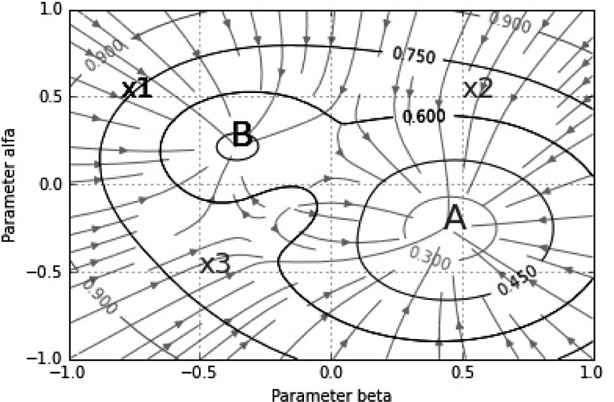
\includegraphics[width=10cm]{images/train_and_loss/non_convex_2.jpg}
%			%\caption{Stripe Radar for Fraud Detection}
%		\end{figure}
		
	%\end{block}

\end{frame}



\begin{frame}
	
	\frametitle{Soluzioni ai problemi di scala: {\color{GradientDescentDiagramBlue}``sottocampionatura''}}
	
	\begin{block}{Sottocampionatura \textit{\textbf{casuale}}}
		Quando la \textbf{campionatura} viene eseguita in modo \textbf{casuale}, il campione viene creato \textbf{scegliendo casualmente gli esempi} che fanno parte del campione: \textbf{più ampio è il campione, maggiore è la probabilità che la campionatura riproduca la struttura e la varietà di dati originali}; ma anche con campioni più piccoli i risultati spesso appaiono accettabili, sia in termini di rappresentazione dei dati originali sia per gli scopi del machine learning.		
	\end{block}

\end{frame}


\begin{frame}
	
	\frametitle{Soluzioni ai problemi di scala: {\color{GradientDescentDiagramBlue}``sottocampionatura''}}
	
	\begin{block}{Sottocampionatura \textit{\textbf{stratificata}}}
		
		Nella \textbf{campionatura stratificata} siete voi a \textbf{controllare la distribuzione finale della variabile obiettivo o di determinate feature nei dati che ritenete fondamentali} per replicare correttamente le caratteristiche dei dati completi. Un esempio classico consiste, al fine di calcolare l’altezza media, nel prelevare un campione in una classe costituita da maschi e femmine \textbf{presenti in proporzioni diverse}.
		\newlinedouble
		Se in media le femmine sono più basse dei maschi e sono presenti in proporzioni inferiori, il campione da estrarre dovrebbe replicare la stessa proporzione se volete ottenere una stima affidabile dell’altezza media, ma questo non è affatto garantito da un’estrazione casuale. Infatti, se per caso estraete un campione composto solo di maschi, finirete per sovrastimare l’altezza media.
		
	\end{block}

\end{frame}


\subsubsection[Parallelismo di rete]{Parallelismo di rete}
\begin{frame}
	
	\frametitle{Soluzioni ai problemi di scala: {\color{GradientDescentDiagramRed}``parallelismo di rete''}}
	
	%\begin{block}{}
		Oltre alla sottocampionatura, esiste una \textit{seconda} soluzione possibile per far stare i dati in memoria, ossia sfruttare il \textbf{parallelismo di rete}, che suddivide i dati fra più computer connessi in rete.
		\textbf{Ciascun computer gestisce una parte dei dati} per l’ottimizzazione; quando ogni computer ha terminato i propri calcoli e tutte le attività di ottimizzazione \textbf{vengono riconvogliate} in un singolo calcolatore, significa che è stata raggiunta una soluzione.
		\newlinedouble
		Questo approccio sta alla base della tecnologia map-reduce e dei \textbf{framework cluster-computer}, Apache Hadoop e Apache Spark.\\
		%, la cui strategia consiste nel mappare (map) un problema su più macchine riducendo (reduce) infine l’output alla soluzione desiderata. 
		Tuttavia \textbf{non} è facile, purtroppo, suddividere \textbf{tutti gli algoritmi} di machine learning in processi separati, problema che limita la possibilità di adottare sempre questo approccio.\\
		Per di più, quando si deve installare e mantenere una rete di computer pronta a svolgere questo tipo di elaborazione dei dati ci si trova ad affrontare \textbf{costi e sprechi di tempo notevoli}.
		%, il che limita l’applicabilità di questo approccio solo alle grandi organizzazioni.
	%\end{block}

\end{frame}


\subsubsection[Algoritmi out-of-core]{Algoritmi out-of-core}
\begin{frame}
	
	\frametitle{Soluzioni ai problemi di scala: {\color{GradientDescentDiagramGreen}``algoritmi out-of-core''}}	
	%\begin{block}{}
		Una \textit{terza} soluzione consiste nel basarsi su \textbf{algoritmi out-of-core}, che mantengono i dati su un dispositivo di memorizzazione, passandone quindi delle porzioni (\textbf{chunk}) alla memoria del computer quando devono essere elaborati; questo processo di passaggio dei dati prende il nome di \textbf{streaming}.
		\newlinedouble
		Poiché i chunk sono più piccoli della memoria centrale, l’algoritmo riesce a gestirli correttamente e a utilizzarli per aggiornare l’ottimizzazione dell’algoritmo di machine learning. Dopo l’aggiornamento, il sistema scarta i chunk vecchi in favore di quelli nuovi, che vengono impiegati dall’algoritmo per imparare. Il processo prosegue più volte finché non ci sono più chunk.
	%\end{block}

\end{frame}


\begin{frame}
	
	\frametitle{Soluzioni ai problemi di scala: {\color{GradientDescentDiagramGreen}``algoritmi out-of-core''}}	
	\begin{block}{Apprendimento mini-batch e online}
		
		Per gli algoritmi out-of-core si parla di due differenti approcci:
		\begin{itemize}
			\item \textbf{apprendimento mini-batch}: se la dimensione dei chunk viente ridotta, in funzione della memoria centrale
			\item \textbf{apprendimento online}: se i chunk sono costituiti da un singolo esempio
		\end{itemize}
	\end{block}

\end{frame}